\section{A Peek into the Implementation Details}
\label{sec:implementation}

As previously mentioned, the framework we present here relies on the one hand on
DSL composition, and on the other hand on a process to guide the user through
the construction of a model. The most important blocks for defining a
process are \emph{properties} of the composed model being defined. These
properties extend an internal MPS Java \textsf{BaseLanguage} interface (defined
at the metameta M3 level), called \textsf{SpecificChecker}.
The  \textsf{SpecificChecker} interface is implemented by all model checkers
inside MPS. A few model checkers are already implemented inside MPS for
analyzing models and returning error instances. Those model checkers
search for example for typing errors or metamodel constraint violations. We
extend the same \textsf{SpecificChecker} interface in order to build our custom checkers that
can perform arbitrary checks on models, including interfacing with external
analyzers. We then wrap such checkers using concepts of the \textsf{Property}
language (see figure~\ref{fig:model_reqs}) to build the \emph{properties} which
are in turn used by the processes defined as instances of the \textsf{Process}
language.

The \emph{domain specific tool developer} is responsible for configuring the
process that will be used by the dashboard to provide hints to the final user.
This process is built as a instance of the \textsf{Process} language. An example
of such an instance can be observed in figure~\ref{fig:flow_model}, including the
first two states of the process for gathering requirements for cooling
controllers.

\begin{figure*}[!h]
\centering 
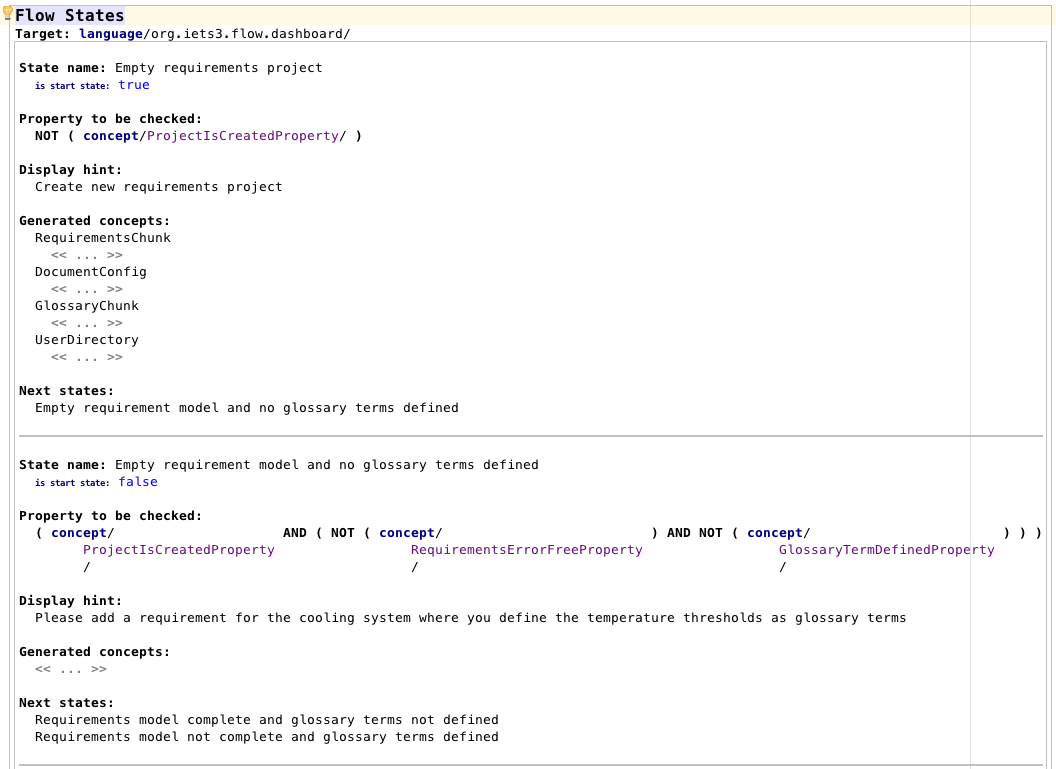
\includegraphics[width=1.55\columnwidth]{./figures/FlowModel.png}
\caption{An sample of the instance of the Flow language for the cooling
controller example}
\label{fig:flow_model}
\end{figure*}

A process model contains states, where for each state the  \emph{domain
specific tool developer} needs to define the type of state (\emph{start},
\emph{intermediate} or \emph{final}), its name, the \emph{condition} to be
checked on the model, the text that should be displayed in the hint box on the
dashboard, the new instances of concepts to be generated, if any, and the next
states. The \emph{condition} of a state is built as a propositional logic
formula having as propositions concepts of the \textsf{Property} language, that are to
be checked on the requirements model. Note that it is also possible to declare in a process
state that data is copied from existing parts of the model onto the new
instances that are created in case the hint is \emph{creational}.

Once a process as been defined, the \emph{domain specific tool developer} can
then use an MPS intention to copy the process data in
figure~\ref{fig:flow_model} to the \textsf{Dashboard} language declared as the
\emph{target} at the top of figure~\ref{fig:flow_model}. This makes it such that
the \textsf{Dashboard} language becomes aware of the process to be used for the
model-driven development environment being built.

When a new dashboard is created in a project as an instance of the
\textsf{Dashboard} language, an algorithm will continuously run in the
background for calculating the current state of the process of creation of the composed model.
This algorithm relies on the fact that the process graph has the following
properties: it is a directed acyclic graph, having only one \emph{start state}
and one \emph{end state}. Additionally, we also assume that forks imply
different paths to achieve the same goal. This is enforced by mutually
exclusive conditions on the  states that follow a fork. As an example, in
figure~\ref{fig:flow_statechart} it can be seen that the requirements model can be completed before the glossary terms are introduced, or
the other way around. However, both must be finished before the ``Requirements
Model Complete and Glossary Defined'' state. A corollary of this assumption 
is that only one state at a time can be the current state in the process
graph flow.

The algorithm that calculates the current state operates by starting at the
initial state and following the flow model graph until no more states can be
found that satisfy the model. The last state that satisfies the model is
returned as the current state. By skipping intermediate states that evaluate to
\emph{true} we avoid stopping the search at states of the process which will
always be satisfied by the composed model after a given point, such as the
``Requirement Model Complete and Glossary Terms Defined'' state in our running
example.
% Note that this algorithm accomodates the fact that properties stated in already
% visited states in the process may evaluate to \emph{false} once the user
% advances in the construction of the composed model. An example of one of such
% conditions is the formula for the ``Empty requirements project'' state in figure~\ref{fig:flow_model}, which is the
% negation of the property that the project exists. Naturally, once the project is
% created this condition will become \emph{false}. When searching for the
% current state, the algorithm skips states that evaluate to \emph{false}.

The main advantage of this algorithm we present here is that it allows for the
current state to go backwards if parts of the model are deleted, as the process
is always searched from the start. However, given our semantics of always
returning for the latest state which property is satisfied by the model, care
should be taken when designing the conditions on states. In particular,
deletions in the model should not lead to inconsistencies between the current
state as reported by the dashboard and the real current state.\levi{talk about
extrapolating the algorithm to multiple end states and multiple current states}

The running example we have described in this paper can be downloaded
at~\cite{coolingControllerProcess} as an MPS project. Another case study of
using our framework is available at~\cite{earsctrlProcess}, where we have
designed a process to assist the user in building natural langage-like
requirements for embedded controllers. This second case study is based on the
work we have previously implemented on the EARS-CTRL tool~\cite{NFM17} and it
features properties in the process definition that are analysed by interfacing
with the  external~\textsf{autoCode4}~\cite{autoCode17} tool. Note that
both~\cite{coolingControllerProcess,earsctrlProcess} are GitHub repositories
that contain not only MPS projects, but also additional information about how to
install those projects as well and pointers to videos demonstrating the usage of
our framework.

% DSL composition is achieved using MPS' native
% mechanisms where references to objects of a DSL can simply be embedded in
% objects of another DSL. This can be observed for example in
% figure~\ref{fig:new_req}, where the ``RequirementsConfig'' object that
% defines some metadata for the project is refered to from an object where a
% requirement is defined.
